\documentclass{beamer}

\usepackage{filecontents}

\newcommand{\compit}[1]{\immediate\write18{pdflatex -synctex=1 -interaction=nonstopmode #1.tex; rm #1.aux #1.log #1.synctex.gz #1.tex}}

\begin{filecontents*}{hiddenlayout.tex}
	\documentclass[preview,border=12pt,12pt]{standalone}
	\usepackage[a6paper,margin=1cm,showframe]{geometry}
	\usepackage{lipsum}
	\begin{document}
		\section*{Minipage}
		\noindent
		\fbox{%
		\begin{minipage}{.45\linewidth}
		hats
		\end{minipage}}
		\hfill
		\fbox{
		\begin{minipage}{.45\linewidth}
		Right Minipage
		\end{minipage}}
		
		\section*{Hello World}
		{\tiny\lipsum[1]}
	\end{document}
\end{filecontents*}

\compit{hiddenlayout}

\begin{filecontents*}{hiddensimplestdoc.tex}
	\documentclass{article}
	\usepackage{lipsum}
	\title{The simplest}
	\author{Wes Honeycutt}
		\begin{document}
			\maketitle
			\lipsum[1]
		\end{document}
\end{filecontents*}

\compit{hiddensimplestdoc}

\begin{filecontents*}{hiddentitlearticle.tex}
	\documentclass{article}
	\usepackage{lipsum}
	\title{The Pitfalls of LaTeX}
	\author{
		Wesley T. Honeycutt
		\thanks{University of Oklahoma Department of Biology}
		\and Leon the Cat}
	\subtitle{Stack Exchange was down and other horror stories}
	\subject{A Joke Paper}
	\begin{document}
		\maketitle
		\lipsum[1]
	\end{document}
\end{filecontents*}

\compit{hiddentitlearticle}


\begin{filecontents*}{hiddentitlescrbook.tex}
	\documentclass{scrbook}
	\usepackage{lipsum}
	\title{The Pitfalls of LaTeX}
	\author{
		Wesley T. Honeycutt
		\thanks{University of Oklahoma Department of Biology}
		\and Leon the Cat}
	\subtitle{Stack Exchange was down and other horror stories}
	\subject{A Joke Paper}
	\begin{document}
		\maketitle
		\lipsum[1]
	\end{document}
\end{filecontents*}

\compit{hiddentitlescrbook}


\begin{filecontents*}{hiddentitlereport.tex}
	\documentclass{report}
	\usepackage{lipsum}
	\title{The Pitfalls of LaTeX}
	\author{
		Wesley T. Honeycutt
		\thanks{University of Oklahoma Department of Biology}
		\and Leon the Cat}
	\subtitle{Stack Exchange was down and other horror stories}
	\subject{A Joke Paper}
	\begin{document}
		\maketitle
		\lipsum[1]
	\end{document}
\end{filecontents*}

\compit{hiddentitlereport}


\begin{filecontents*}{hiddentitleelsarticle.tex}
	\documentclass{elsarticle}
	\usepackage{lipsum}
	\title{The Pitfalls of LaTeX}
	\author{
		Wesley T. Honeycutt
		\thanks{University of Oklahoma Department of Biology}
		\and Leon the Cat}
	\subtitle{Stack Exchange was down and other horror stories}
	\subject{A Joke Paper}
	\begin{document}
		\maketitle
		\lipsum[1]
	\end{document}
\end{filecontents*}

\compit{hiddentitleelsarticle}

\usepackage{xcolor}
\usepackage{fontawesome}
\usepackage{tikz}
	\usetikzlibrary{patterns}
\usepackage{hologo}
\usepackage{showexpl}
\usepackage{hyperref}
\usepackage{calc}
\usepackage{fp}

\title{An Introduction to \LaTeX}
\subtitle{Make Documents Like A PROgrammer}
\author{Wesley T. Honeycutt}
\institute{University of Oklahoma}
\date{\today}

\makeatletter
\Hy@AtBeginDocument{%
	\def\@pdfborder{0 0 1}% Overrides border definition set with colorlinks=true
	\def\@pdfborderstyle{/S/U/W 1}% Overrides border style set with colorlinks=true
	% Hyperlink border style will be underline of width 1pt
}
\makeatother

\hypersetup{%
	colorlinks=true,% hyperlinks will have color
	linkcolor=blue,
	urlcolor=blue,
	linkbordercolor=blue,% hyperlink borders will be red
	pdfborderstyle={/S/U/W 1}% border style will be underline of width 1pt
}

\lstloadlanguages{[LaTeX]Tex} 
\lstset{%
	tabsize=2, % Our tabs will be displayed with 2 spaces each
	gobble=6, % We gobble the first x characters (removes excess tabs)
	basicstyle=\ttfamily\scriptsize,
	commentstyle=\itshape\ttfamily\scriptsize,
	showspaces=false,
	showstringspaces=false,
	breaklines=true,
	breakautoindent=true,
	captionpos=t
} 

\newcommand{\metalone}{[pattern= horizontal lines, pattern color=blue]}
\newcommand{\metaltwo}{[pattern= vertical lines, pattern color=purple]}
\newcommand{\poly}{[pattern= grid, pattern color=red]}
\newcommand{\pdiff}{[pattern= north east lines, pattern color=orange]}
\newcommand{\ndiff}{[pattern= north west lines, pattern color=green]}
\newcommand{\pwell}{[pattern= crosshatch dots, pattern color=orange]}
\newcommand{\nwell}{[pattern= crosshatch dots, pattern color=green]}
\newcommand{\oxide}{[pattern = bricks, pattern color = olive]}
\newcommand{\silicon}{[fill = white]}
\newcommand{\metalthree}{[fill = teal]}

\begin{document}

	\frame{\titlepage}
	
	\frame{\frametitle{If you want to follow along}
		\href{https://github.com/BlueNalgene/Introduction_to_LaTeX}{https://github.com/BlueNalgene/Introduction\_to\_LaTeX}	
	}
	
	\section{What in the world is \LaTeX}
	
		\frame{\frametitle{History}
			In 1978, Donald Knuth created the \TeX\ programming language in a fit of frustration with how ugly photoprinting looked.
			\\~\\
			In 1983, Leslie Lamport released \LaTeX\ (Layman's \TeX), a set of macros which made \TeX\ usable by mortals.
			\\~\\
			There are many other variants such as :
			\begin{center}
				\hologo{BibTeX}\ \hologo{ConTeXt}\ \hologo{LuaTeX}\ \hologo{LyX}\ \hologo{pdfLaTeX}\ \hologo{XeLaTeX}
			\end{center}
		}
	
		\begin{frame}{\LaTeX~is\ldots}
			\ldots a sophisticated document preparation sytem.
			\\~\\
			\begin{block}{\LaTeX~has\ldots}
				\begin{itemize}
					\item Stylistic uniformity
					\item Bibliography support
					\item Sophisticated structuring abilities
					\item Reference tracking
					\item Highly extendible capabilities
				\end{itemize}
			\end{block}
		\end{frame}
		
		\begin{frame}{\LaTeX~is not\ldots}
			\ldots a word processor.
			\\~\\
			\begin{block}{\LaTeX~does not\ldots}
			\begin{itemize}
				\item Spell-check your documents
				\item Give you complete control over formatting
				\item Provide a graphical interface for editing
			\end{itemize}
			\end{block}
			``You take care of writing, and we'll take care of presentation."
		\end{frame}
	
		\frame{\frametitle{You might be used to WYSIWYG}
			\begin{center}
				\setlength{\tabcolsep}{0pt}
				\begin{tabular}{cl}
					\textbf{W}&hat \\
					\textbf{Y}&ou \\
					\textbf{S}&ee \\
					\textbf{I}&s \\
					\textbf{W}&hat \\
					\textbf{Y}&ou \\
					\textbf{G}&et
				\end{tabular}
			\end{center}
		}
	
		\frame{\frametitle{\LaTeX is WYSIWYM}
			\begin{center}
				\setlength{\tabcolsep}{0pt}
				\begin{tabular}{cl}
					\textbf{W}&hat \\
					\textbf{Y}&ou \\
					\textbf{S}&ee \\
					\textbf{I}&s \\
					\textbf{W}&hat \\
					\textbf{Y}&ou \\
					\textbf{M}&ean
				\end{tabular}
			\end{center}
		}
	
		\frame[containsverbatim]{\frametitle{Presentation matching what you wrote, not how it was written}
			\begin{LTXexample}
				This     text is 
				spaced      specially.
			\end{LTXexample}
	
			\begin{LTXexample}<2>
				Paragraphs are easy.
				
				Use double line breaks.
			\end{LTXexample}

			\begin{LTXexample}
				Never break the unbreakable unless you want to.  
				
				You~can~force~connections~of~words~in~a~line~or\ force\ spaces and\\linebreaks.
			\end{LTXexample}
		}
	
	\section{Compilers}
	
		\frame[containsverbatim]{\frametitle{If you like to suffer}
			\LaTeX{}is coded as plaintext.  If you really want to, you can do everything in a Notepad-like text editor.
			\\~\\
			The code is processed via command line:
			\begin{lstlisting}
				pdflatex thefile.tex
			\end{lstlisting}
		}
	
		\frame{\frametitle{There are add-ons for popular text editors}
			\begin{itemize}
				\item<1-> \textit{vim}: \href{http://vim-latex.sourceforge.net}{\LaTeX{}suite for vim}
				\item<2-> \textit{emacs}: \href{http://personal.psu.edu/jcc8//software/latexmk-jcc/}{Latexmk}
				\item<3-> \textit{Notepad++}: \href{http://johnbruer.com/2013/05/21/latex-editing-using-notepad/}{Requires multiple tweaks}
				\item<4-> \textit{Sublime Text}: \href{https://latextools.readthedocs.io/en/latest/}{\LaTeX{}Tools}
				\item<5-> \textit{Atom}: \href{https://atom.io/packages/latex}{\LaTeX{}apm}
			\end{itemize}
		}
	
		\frame{\frametitle{Lots of \LaTeX{} IDE's}
			\begin{columns}[onlytextwidth,T]
				\column{\linewidth/2-\linewidth/20}
				\begin{itemize}
					\item<1-> TeXstudio \faWindows{} \faApple{} \faLinux{}
					\item<2-> Texmaker \faWindows{} \faApple{} \faLinux{}
					\item<3-> LyX \faWindows{} \faApple{} \faLinux{}
					\item<4-> MacTeX \faApple{}
					\item<5-> MiKTeX \faWindows{}
					\item<6-> TeX Live \faLinux{}
				\end{itemize}
				\column{\linewidth/2-\linewidth/20}
				
				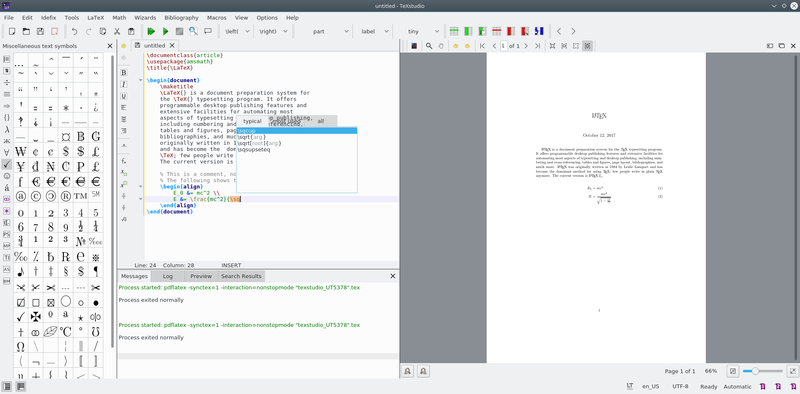
\includegraphics[width=\linewidth]{texstudio.png}<1>
				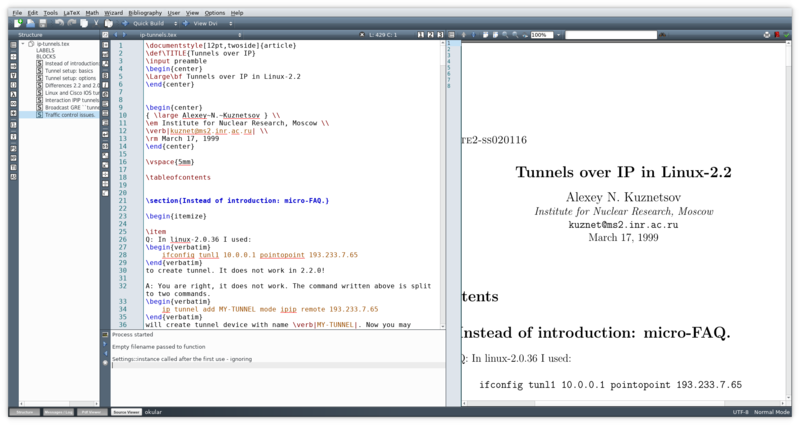
\includegraphics[width=\linewidth]{texmaker.png}<2>
				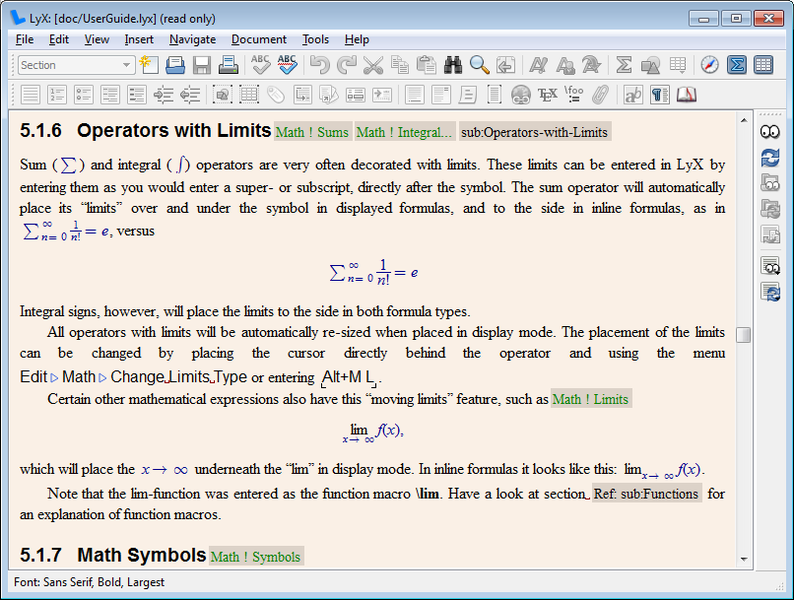
\includegraphics[width=\linewidth]{lyx.png}<3>
				
\includegraphics[width=\linewidth]{mactex.png}<4>
				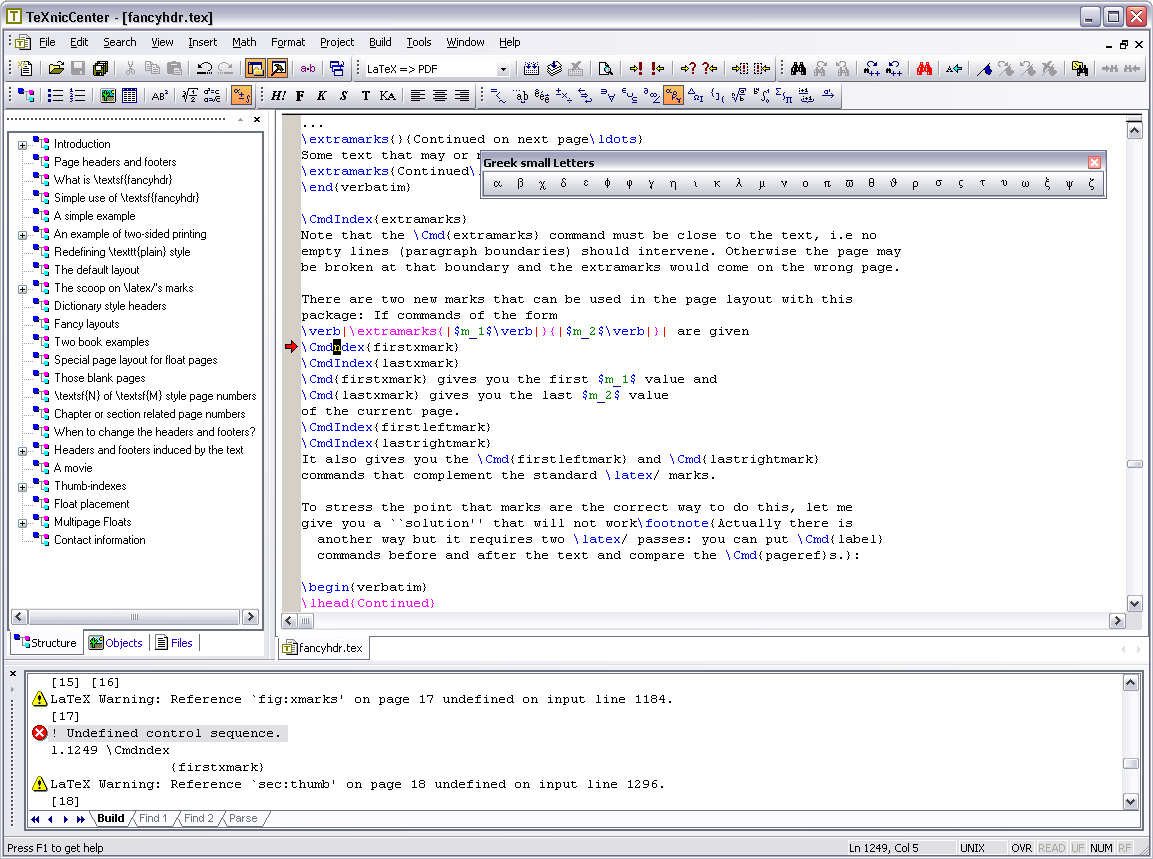
\includegraphics[width=\linewidth]{miktex.png}<5>
			\end{columns}
		}
	
		\frame{\frametitle{Online collaborative options}
			\begin{columns}[onlytextwidth,T]
				\column{\linewidth/2-\linewidth/20}
				\begin{itemize}
					\item<1-> Overleaf/ShareLaTeX
					\item<2-> Authorea
					\item<3-> There are others which I have no experience with.
				\end{itemize}
				\column{\linewidth/2-\linewidth/20}
				
				
\includegraphics[width=\linewidth]{overleaf.png}<1>
				
\includegraphics[width=\linewidth]{authorea.jpg}<2>
			\end{columns}
			
		}
	
	
	\section{The Basics and Principles}
		\frame{\frametitle{Learn to love braces}
			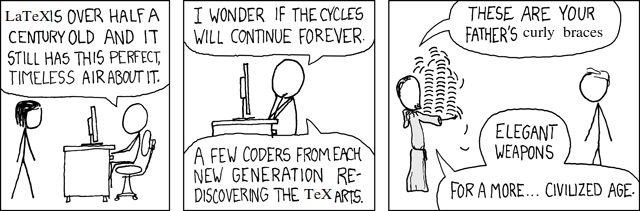
\includegraphics[width=\textwidth-5pt]{xkcd.png}
			
			\footnotetext{With apologies to Randall Munroe}
		}
	
		\frame[containsverbatim]{\frametitle{Commands and Environments}
			\begin{LTXexample}
				Uncentered
			\end{LTXexample}
			
			\begin{LTXexample}
				\begin{center}
					Centered Environment
				\end{center}
			\end{LTXexample}
		
			\begin{LTXexample}
				\centering
				Command Centered
			\end{LTXexample}
		}
	
		\frame{\frametitle{The Logical Structure of a \LaTeX\ Document}
			\begin{block}{Preamble}
				\begin{itemize}
					\item<1-> Declare the document type you will be making: \\
					\textbackslash{}documentclass[options]\{class\}
					\item<2-> Declare what packages you will need: \\
					\textbackslash{}usepackage[options]\{package\}
					\item<3-> Define any custom functions or environments
					\item<4-> Declare important variables
				\end{itemize}
			\end{block}
		}
	
		\frame{\frametitle{The Logical Structure of a \LaTeX\ Document cont'd}
			\begin{block}{Body}
				\begin{itemize}
					\item<1-> Initialize the document in an environment\\
					\textbackslash{}begin\{document\}\\
					\qquad\ldots\\
					\textbackslash{}end\{document\}
					\item<2-> Within this environment you will:
					\begin{itemize}
						\item<3-> Create the title page or section:\\
						\textbackslash{}maketitle
						\item<4-> Write your document
					\end{itemize}
				\end{itemize}
			\end{block}
		}
	
		\frame[containsverbatim]{\frametitle{The simplest document}
			\begin{columns}[onlytextwidth,T]
				\column{\linewidth/2-5mm}
				{%
					\setlength{\fboxsep}{0pt}%
					\setlength{\fboxrule}{1pt}%
					\fbox{\includegraphics[width=\linewidth]{hiddensimplestdoc}}
				}\\
				\column{\linewidth/2-5mm}
					\begin{lstlisting}
			\documentclass{article}
			\usepackage{lipsum}
			\title{The simplest}
			\author{Wes Honeycutt}
			\begin{document}
				\maketitle
				\lipsum[1]
			\end{document}
					\end{lstlisting}
			\end{columns}
		}
	
		\frame{\frametitle{Making the \textbackslash{}maketitle}
			The title can include several elements, which are declared by the user.
			\begin{itemize}
				\item<2-> \textbackslash{}title\{The Title\}
				\item<3-> \textbackslash{}author\{The Author's Name\}
					\begin{itemize}
						\item<4-> This can include \textbackslash{}thanks\{Some Institution\}
					\end{itemize}
				\item<5-> \textbackslash{}subtitle\{A Clever Subtitle\}
				\item<6-> \textbackslash{}subject\{A Subject Heading\}
			\end{itemize}
		}
	
		\frame[containsverbatim]{\frametitle{Our Sample Title Page}
			\begin{lstlisting}
				\title{The Pitfalls of LaTeX}
				
				\author{
					Wesley T. Honeycutt
					\thanks{University of Oklahoma Department of Biology} 
					\and Leon the Cat}
					
				\subtitle{Stackexchange was down and other horror stories}
				
				\subject{A Joke Paper}
			\end{lstlisting}
		}
	
		\frame{\frametitle{\textbackslash{}documentclass\{article\}}
			\begin{columns}[onlytextwidth,T]
				\column{\linewidth/2-\linewidth/20}
				\includegraphics[width=\linewidth, page=1]{hiddentitlearticle}
				\column{\linewidth/2-\linewidth/20}
				\includegraphics[width=\linewidth, page=2]{hiddentitlearticle}
			\end{columns}	
		}
	
		\frame{\frametitle{\textbackslash{}documentclass\{scrbook\}}
			\begin{columns}[onlytextwidth,T]
				\column{\linewidth/2-\linewidth/20}
				\includegraphics[width=\linewidth, page=1]{hiddentitlescrbook}
				\column{\linewidth/2-\linewidth/20}
				\includegraphics[width=\linewidth, page=2]{hiddentitlescrbook}
			\end{columns}	
		}
	
		\frame{\frametitle{\textbackslash{}documentclass\{report\}}
			\begin{columns}[onlytextwidth,T]
				\column{\linewidth/2-\linewidth/20}
				\includegraphics[width=\linewidth, page=1]{hiddentitlereport}
				\column{\linewidth/2-\linewidth/20}
				\includegraphics[width=\linewidth, page=2]{hiddentitlereport}
			\end{columns}
		}
	
		\frame{\frametitle{\textbackslash{}documentclass\{elsarticle\}}
			\begin{columns}[onlytextwidth,T]
				\column{\linewidth/2-\linewidth/20}
				\includegraphics[width=\linewidth, page=1]{hiddentitleelsarticle}
				\column{\linewidth/2-\linewidth/20}
				\includegraphics[width=\linewidth, page=2]{hiddentitleelsarticle}
			\end{columns}
		}
	
		\frame{\frametitle{Publisher Distributed Classes}
			\only<1->{The previous example shows how different classes rearrange the same elements.}
			
			
			\begin{block}<2->{Academic Publishers}
				\begin{center}
					Elsevier - $elsarticle$\\
					Springer - $llncs$\\
					IEEE - $IEEEtran$\\
					AMS - $amscls$
				\end{center}
			\end{block}
		}
	
		\frame{\frametitle{Some More Academic Publishers With Classes}
			\begin{itemize}
				\item aaai www.aaai.org
				\item AAAS/science www.sciencemag.org
				\item American Chemical Society Publications
				\item Addison-Wesley
				\item algebra universalis
				\item American Institute of Physics www.aip.org
				\item American Meteorological Society www.ametsoc.org
				\item American Physical Society authors.aps.org
				\item Beech Stave Press
				\item Birkhäuser
				\item Cambridge University Press
				\item CRC
				\item Documenta Mathematica www.math.uiuc.edu
				\item Docscape
				\item Engine House Books
				
			\end{itemize}
		}
		
		\frame{\frametitle{Some More Academic Publishers With Classes}
			\begin{itemize}
				\item Fondo de Cultura Económica
				\item Informs joc.pubs.informs.org
				\item Institut Mittag-Leffler (Royal Swedish Academy of Sciences)
				\item www.arkivformatematik.org
				\item IOP (institute of physics) authors.iop.org
				\item John Benjamins Publishing Company
				\item London Mathematical Society books www.lms.ac.uk
				\item Louisiana State University Press
				\item Mathematical Association of America www.maa.org
				\item National Research Council of Canada
				\item Oxford University Press www.oup.co.uk
				\item Princeton University Press press.princeton.edu
				\item Publications de l'Institut Mathématique (Beograd) www.emis.de
			\end{itemize}
		}
		
		\frame{\frametitle{Some More Academic Publishers With Classes}
			\begin{itemize}
				\item SAS Institute
				\item SIAM books www.siam.org
				\item Springer math www.springer.com
				\item Springer physics www.springer.com
				\item Thomson Delmar Learning
				\item UIT Cambridge
				\item Unipress (Institute of High Pressure Physics, Polish Academy of Sciences)
				\item www.unipress.waw.pl
				\item University of California Press
				\item Wiley www.wiley.com
				\item William Andrew Publishing
				\item World Scientific
				\item WordTech
			\end{itemize}
		}
	
		
	
	
	
	\section{Important Tools}
		
		
		
		
		\frame{\frametitle{Section Hierarchy}
			\textbackslash{}section\{The Topmost\}
			
			\qquad\textbackslash{}subsection\{A Little Deeper\}
			
			\qquad\qquad\textbackslash{}subsubsection\{Deeper Still\}
			
			\qquad\qquad\qquad\qquad\qquad\qquad\qquad\qquad\ldots
		}
		
		\frame[containsverbatim]{\frametitle{Text Formats}
			\begin{LTXexample}
				Be \textbf{Bold}!\\
				\textit{Italicize}!\\
				\underline{Underline} to accentuate!\\
				Write with \emph{emphasis}!\\
			\end{LTXexample}
		}
		
		\frame[containsverbatim]{\frametitle{Font Size}
			\begin{LTXexample} 
				{\Huge I'm shrinking}\\
				{\huge I'm shrinking}\\
				{\LARGE I'm shrinking}\\
				{\Large I'm shrinking}\\
				{\large I'm shrinking}\\
				{\normalsize I'm shrinking}\\
				{\small I'm shrinking}\\
				{\footnotesize I'm shrinking}\\
				{\scriptsize I'm shrinking}\\
				{\tiny I'm shrinking}\\
			\end{LTXexample}
		}
		
		\frame[containsverbatim]{\frametitle{Lists}
			\begin{LTXexample} 
				\begin{itemize} 
					\item Boomer 
					\item Sooner
					\item Oklahoma
				\end{itemize} 
			\end{LTXexample}
			
			\begin{LTXexample} 
				\begin{enumerate} 
					\item Boomer 
					\item Sooner
					\item Oklahoma
				\end{enumerate} 
			\end{LTXexample}
		}
		
		\frame[containsverbatim]{\frametitle{Nested Lists}
			\begin{LTXexample} 
				\begin{itemize} 
					\item Boomer
					\begin{itemize}
						\item Sooner
					\end{itemize}
					\item Oklahoma
				\end{itemize} 
			\end{LTXexample}
			
			\begin{LTXexample} 
				\begin{enumerate} 
					\item Boomer 
					\begin{enumerate}
						\item Sooner
					\end{enumerate}
					\item Oklahoma
				\end{enumerate} 
			\end{LTXexample}
		}
	
		\frame{\frametitle{Graphics}
		
		}
	
		\frame{\frametitle{Tables}
			
		}
	
		\frame{\frametitle{Math}
			
		}
	
	\section{Some Advanced Features (aka Wes shows off his projects)}
	
	
		\frame[containsverbatim]{\frametitle{Graphics Generation with TikZ}
			High quality vector images can be produced from within LaTeX using a package called TikZ.
			
			Additionally, Inkscape can export TikZ directly.
			
			
		}
	
		\frame[containsverbatim]{
			% This slide breaks indentation convention to fit more on slide.
			\begin{lstlisting}
			\begin{tikzpicture}
			\draw \pdiff (0,.25) -- (0,3) -- (1,3) -- (1,2.5) to [out=270,in=180] (1.5,2) -- (3.75,2) to [out=0,in=270] (4.25,2.5) -- (4.25,3) -- (6.75,3) -- (6.75,2.5) to [out=270,in=180] (7.25,2) -- (9.5,2) to [out=0,in=270] (10,2.5) -- (10,3) -- (11,3) -- (11,.25) -- (0,.25) node [midway,above] {p doped Si};
			\draw \metalthree (0,0) rectangle (11,.25) node [midway, color=white]
			{Si Substrate};
			\draw \oxide (4,3) rectangle (7,4) node [pos=.5,font=\bf\Large] {oxide};
			\draw \metalone (4,4) rectangle (7,4.5);
			\draw \ndiff (4.25,3) -- (1,3) -- (1,2.5) to [out=270,in=180] (1.5,2) -- (3.75,2) to [out=0,in=270] (4.25,2.5) -- (4.25,3) node at (2.625,2.5) [align=center] {n-type};
			\draw \ndiff (10,3) -- (6.75,3) -- (6.75,2.5) to [out=270,in=180] (7.25,2) -- (9.5,2) to [out=0,in=270] (10,2.5) -- (10,3) node at (8.375,2.5) [align=center] {n-type};
			\draw \metalone (1.25,3) rectangle (3,3.5);
			\draw \metalone (8,3) rectangle (9.75,3.5);
			\draw [->] (1,5) node [above] {Source} -- (2.125,3.5);
			\draw [->] (10,5) node [above] {Drain} -- (8.975,3.5);
			\draw [->] (5.5,5) node [above] {Gate} -- (5.5,4.5);
			\node at (5.5,-.5) [align=center] {$V_{GS} < V_{threshold}$};
			\end{tikzpicture}
			\end{lstlisting}	
		}
	
			\frame{\frametitle{MOSFET}
				% General n-type mosfet
				\begin{tikzpicture}
					\draw \pdiff (0,.25) -- (0,3) -- (1,3) -- (1,2.5) to [out=270,in=180] (1.5,2) -- (3.75,2) to [out=0,in=270] (4.25,2.5) -- (4.25,3) -- (6.75,3) -- (6.75,2.5) to [out=270,in=180] (7.25,2) -- (9.5,2) to [out=0,in=270] (10,2.5) -- (10,3) -- (11,3) -- (11,.25) -- (0,.25) node [midway,above] {p doped Si};
					\draw \metalthree (0,0) rectangle (11,.25) node [midway, color=white]
					 {Si Substrate};
					\draw \oxide (4,3) rectangle (7,4) node [pos=.5,font=\bf\Large] {oxide};
					\draw \metalone (4,4) rectangle (7,4.5);
					\draw \ndiff (4.25,3) -- (1,3) -- (1,2.5) to [out=270,in=180] (1.5,2) -- (3.75,2) to [out=0,in=270] (4.25,2.5) -- (4.25,3) node at (2.625,2.5) [align=center] {n-type};
					\draw \ndiff (10,3) -- (6.75,3) -- (6.75,2.5) to [out=270,in=180] (7.25,2) -- (9.5,2) to [out=0,in=270] (10,2.5) -- (10,3) node at (8.375,2.5) [align=center] {n-type};
					\draw \metalone (1.25,3) rectangle (3,3.5);
					\draw \metalone (8,3) rectangle (9.75,3.5);
					\draw [->] (1,5) node [above] {Source} -- (2.125,3.5);
					\draw [->] (10,5) node [above] {Drain} -- (8.975,3.5);
					\draw [->] (5.5,5) node [above] {Gate} -- (5.5,4.5);
					\only<1> {\node at (5.5,-.5) [align=center] {$V_{GS} < V_{threshold}$};}
					\only<2-3> {\node at (5.5,-.5) [align=center] {$V_{GS} \geq V_{threshold}$};
						\node at (5.5,-1) [align=center] {$V_{DS} < V_{GS} - V_{threshold}$};
						}
					\only<3> {\draw [fill=white] (4.25,3) rectangle (6.75,2.5);
						\draw \ndiff (4.25,3) rectangle (6.75,2.5);
						}
					\only<4-5> {\node at (5.5,-.5) [align=center] {$V_{GS} \geq V_{threshold}$};
						\node at (5.5,-1) [align=center] {$V_{DS} = V_{GS} - V_{threshold}$};
						}
					\only<5> {\draw [fill=orange,orange] (4.25,3) rectangle (6.75,2.5);
						\draw [fill=white] (4.25,3) -- (4.25,2.65) -- (6.75,3) -- (4.75,3);
						\draw \ndiff (4.25,3) -- (4.25,2.65) -- (6.75,3) -- (4.75,3);
						}
					\only<6-7> {\node at (5.5,-.5) [align=center] {$V_{GS} \geq V_{threshold}$};
						\node at (5.5,-1) [align=center] {$V_{DS} > V_{GS} - V_{threshold}$};
						}
					\only<7> {\draw [fill=orange,orange] (4.25,3) rectangle (6.75,2.5);
						\draw [fill=white] (4.25,3) -- (4.25,2.85) -- (6.75,3) -- (4.75,3);
						\draw \ndiff (4.25,3) -- (4.25,2.85) -- (6.75,3) -- (4.75,3);
						}
				\end{tikzpicture}
		}
		
		\frame{\frametitle{Super Powerful for Theses}
			% Pop a chapter out, boom... you got a paper.
			
			% OSU doesn't have one.  What a bummer.  I made one myself.
			
			% OU does have one.  Let's link you to it.
			% http://www.math.ou.edu/~mgsa/latex.html
		}
	
		\frame{\frametitle{Make a Custom Class}
			% Show off my fancy executive summary.
			\centering
			
\includegraphics[height=0.9\textheight]{redcedar.pdf}
		}
	
		\frame{\frametitle{Make a Custom Class}
			\centering
			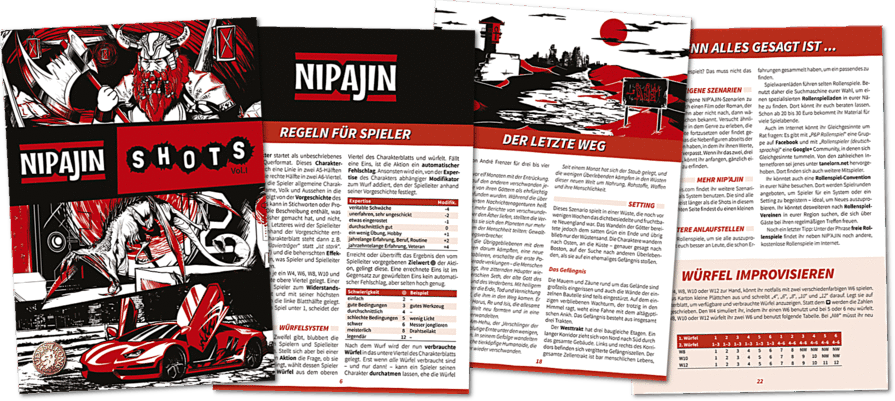
\includegraphics[width=0.9\linewidth]{nipajin.png}\\
			\href{https://github.com/ludus-leonis/nipajin}{https://github.com/ludus-leonis/nipajin}
		}
	
		\frame{\frametitle{Make a Custom Class}
			\centering
			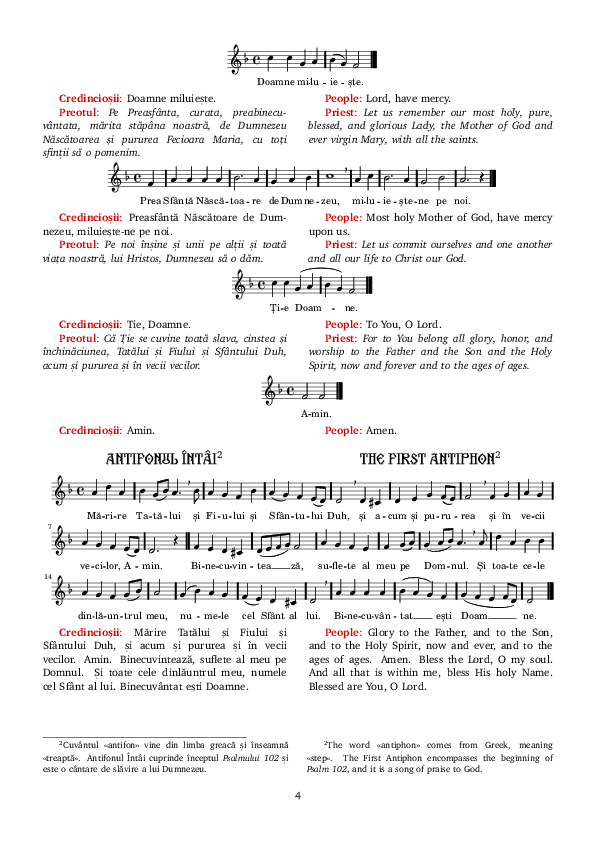
\includegraphics[height=0.8\textheight]{liturghie.png}\\
			\href{http://www.liturghie.net/}{http://www.liturghie.net/}
		}
	
		\frame{\frametitle{Make a Custom Class}
			\centering
			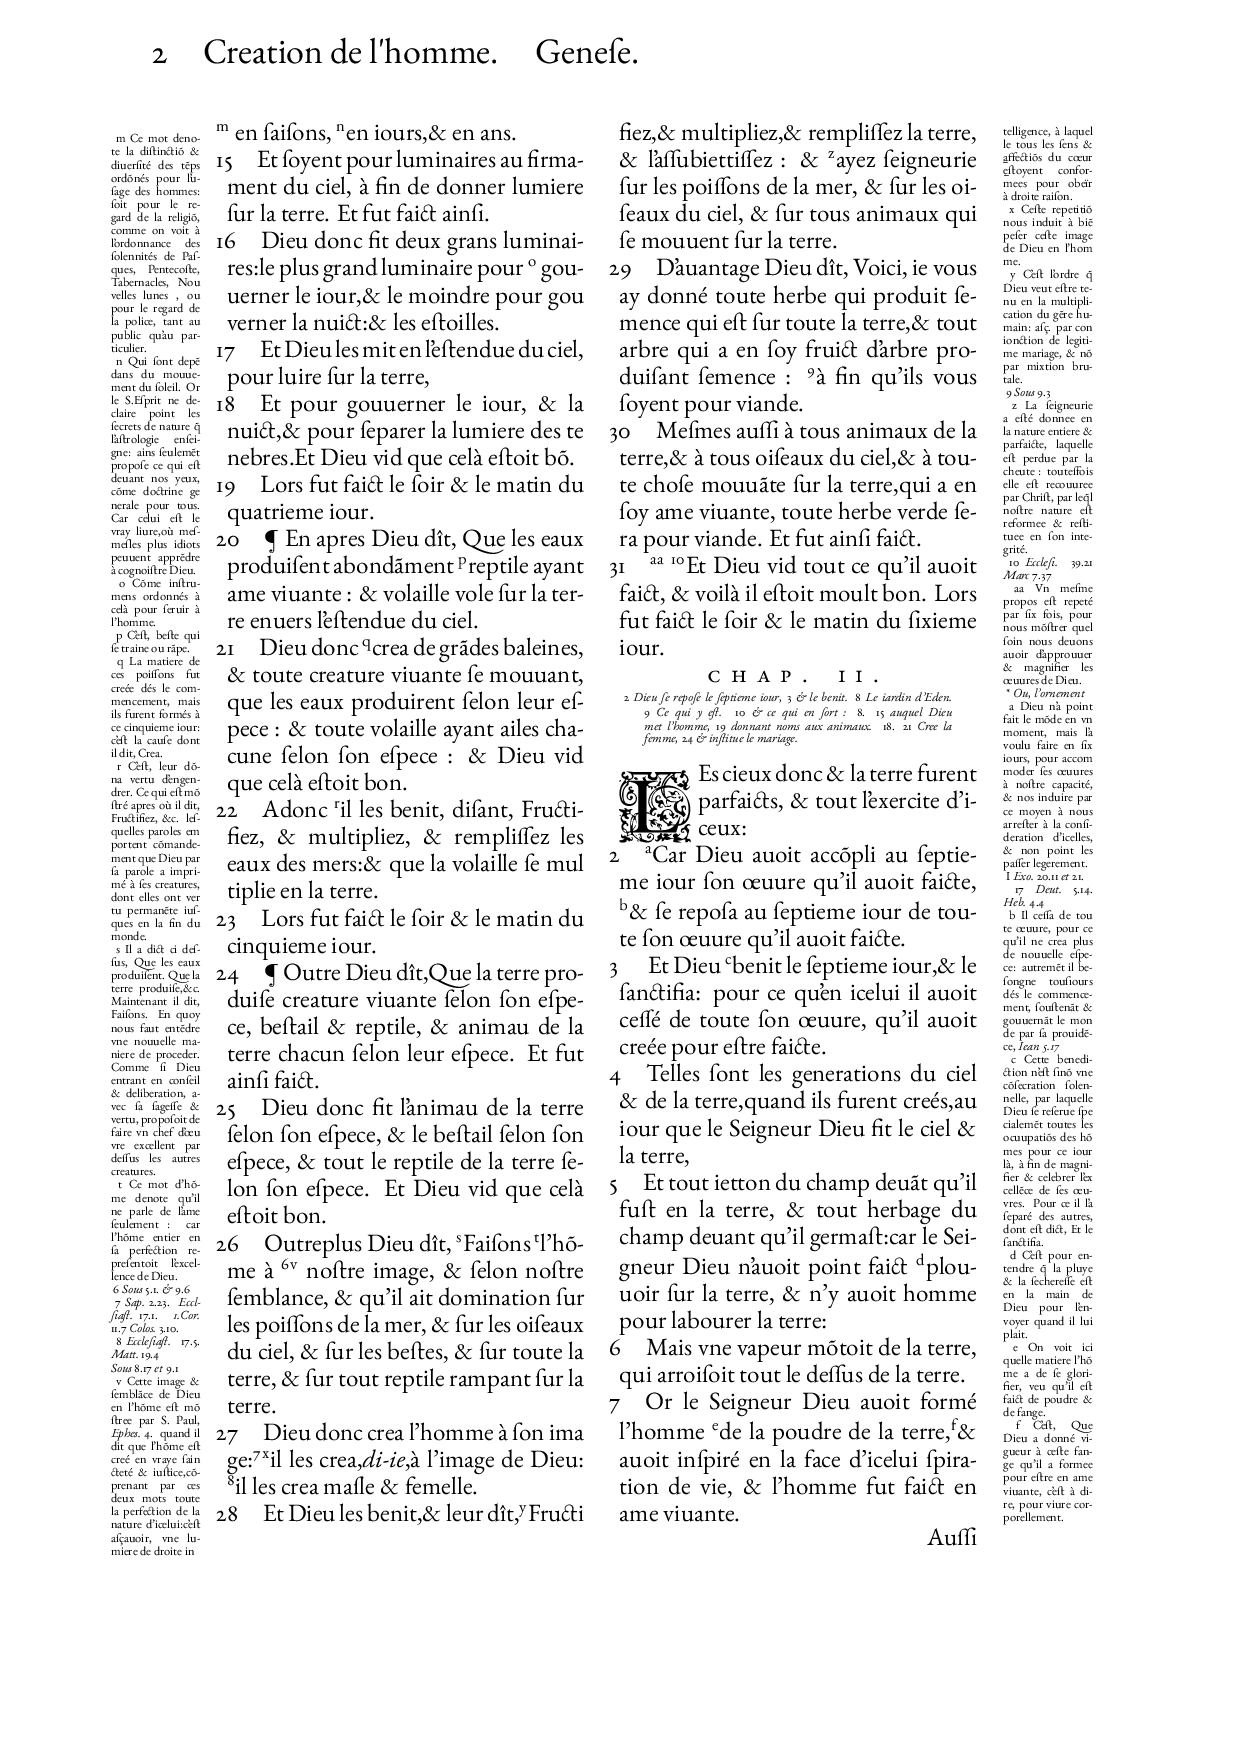
\includegraphics[height=0.75\textheight]{bible.png}\\
			\href{https://github.com/raphink/geneve_1564}{https://github.com/raphink/geneve\_1564}
		}
	
		\frame{\frametitle{Make a Custom Class}
			\centering
			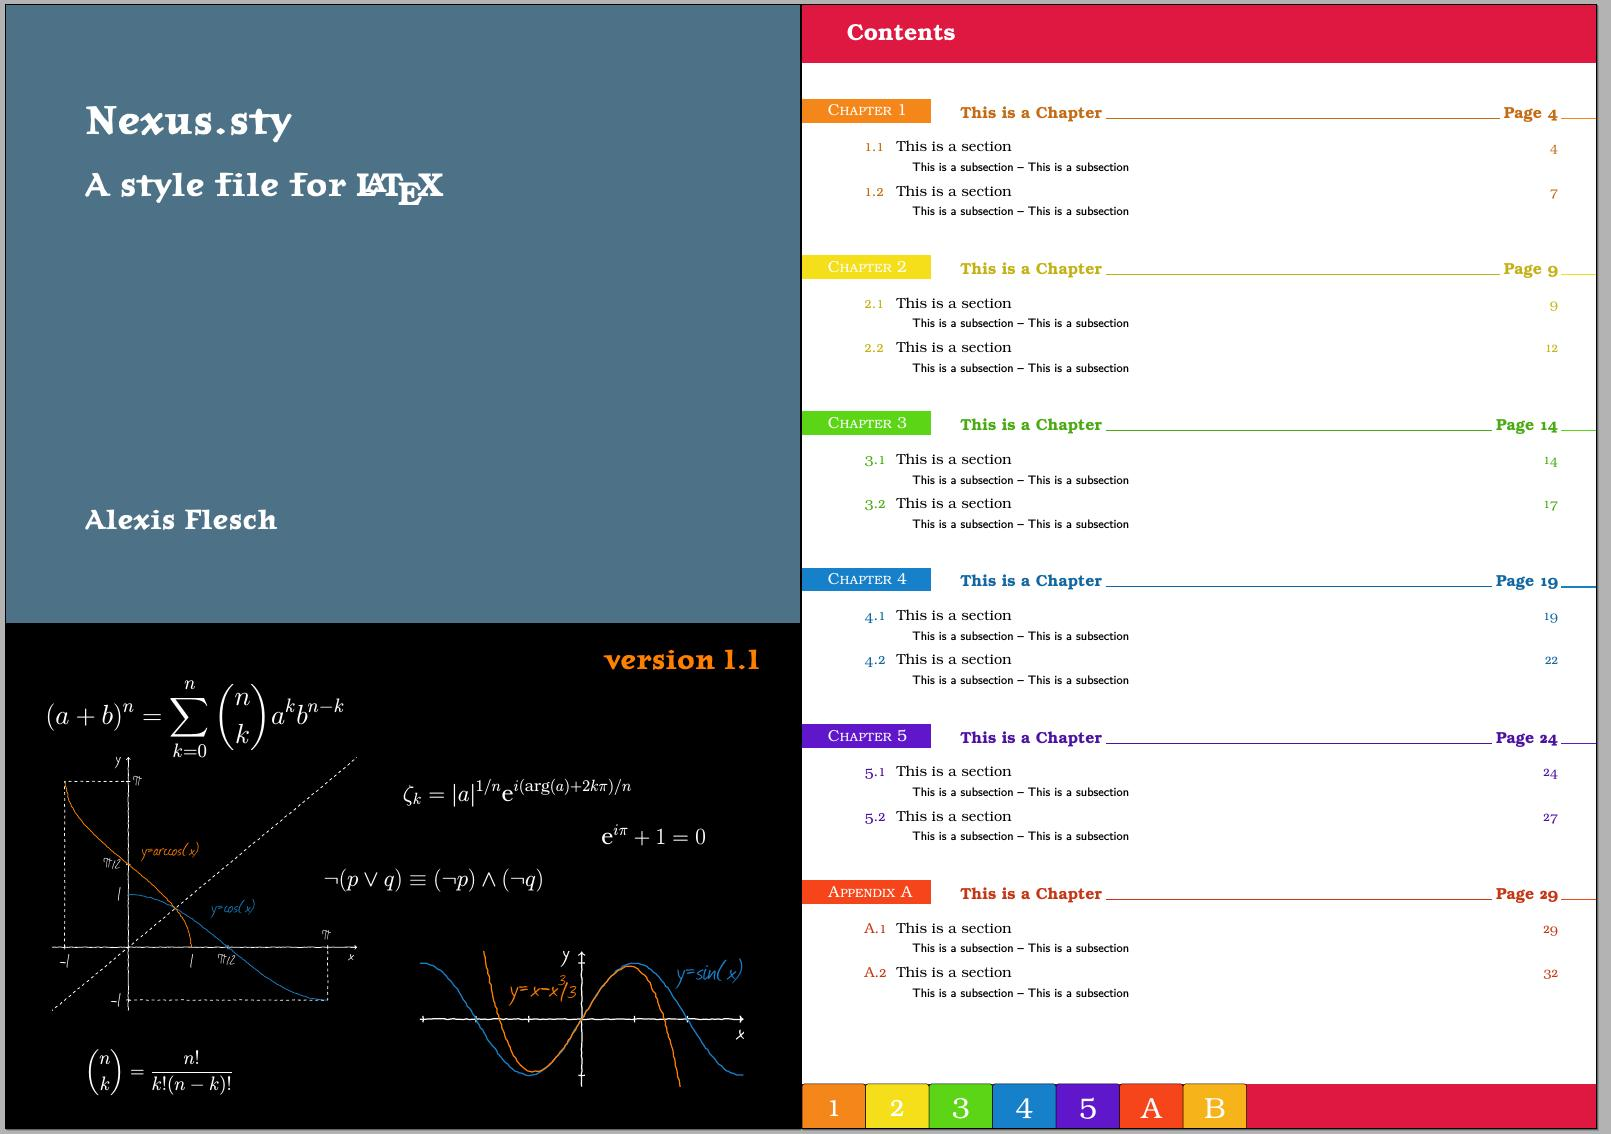
\includegraphics[width=0.9\linewidth]{textbook.jpg}\\
			\href{https://github.com/alexisflesch/nexus}{https://github.com/alexisflesch/nexus}
		}
	
		\frame[containsverbatim]{\frametitle{Unique Words and Hypenation}
			\LaTeX{} automatically hyphenates words in the dictionary.  What if you have something that isn't common?
			\\~\\
			\begin{lstlisting}
				\hyphenation{Red-ce-dar May-ap-ple Ok-la-ho-ma che-mo-ther-apy through}
			\end{lstlisting}
		}
	
		\frame[containsverbatim]{\frametitle{Do calculations}
			\LaTeX{}wasn't made for math, but you do have access to registers \ldots
			\\~\\
			\begin{block}{\textbackslash{}usepackage\{calc\}}
			\begin{LTXexample}
			\newlength{\mylength}
			\setlength{\mylength}{\textwidth}%
			\noindent\rule{\mylength}{20pt}
			
			\bigskip
			\setlength{\mylength}{\textwidth-1cm}%
			\noindent\rule{\mylength}{20pt}
			
			\bigskip
			\setlength{\mylength}{\textwidth-80pt+5mm-1bp}%
			\noindent\rule{\mylength}{20pt}
			\end{LTXexample}
			\end{block}
		}
	
		\frame[containsverbatim]{\frametitle{Do calculations}
			\ldots and floating points.
			\\~\\	
			\begin{block}{\textbackslash{}usepackage\{fp\}}
			\begin{LTXexample}
			The following arithmetic is easy:
			\begin{itemize}
			\item \FPeval{\result}{clip(5+6)}%
			$5+6=\result$
			\item \FPeval{\result}{round(2+3/5*pi,5)}%
			$2+3/5\times\pi=\result$
			\end{itemize}
			\end{LTXexample}
			\end{block}
		}
	
		\frame{\frametitle{I use math for my consulting invoices.}
			\centering
			\includegraphics[height=0.9\paperheight]{hiddeninvoice}
		}
	
	\section{Learning More}
	
		\frame{\frametitle{RTFM}
			
			\begin{columns}[onlytextwidth,T]
				\column{\linewidth/2-5mm}
					The Comprehensive \TeX\ Archive Network is a package repository
					\\~\\
					This also includes manuals and examples
				\column{\linewidth/2-5mm}
					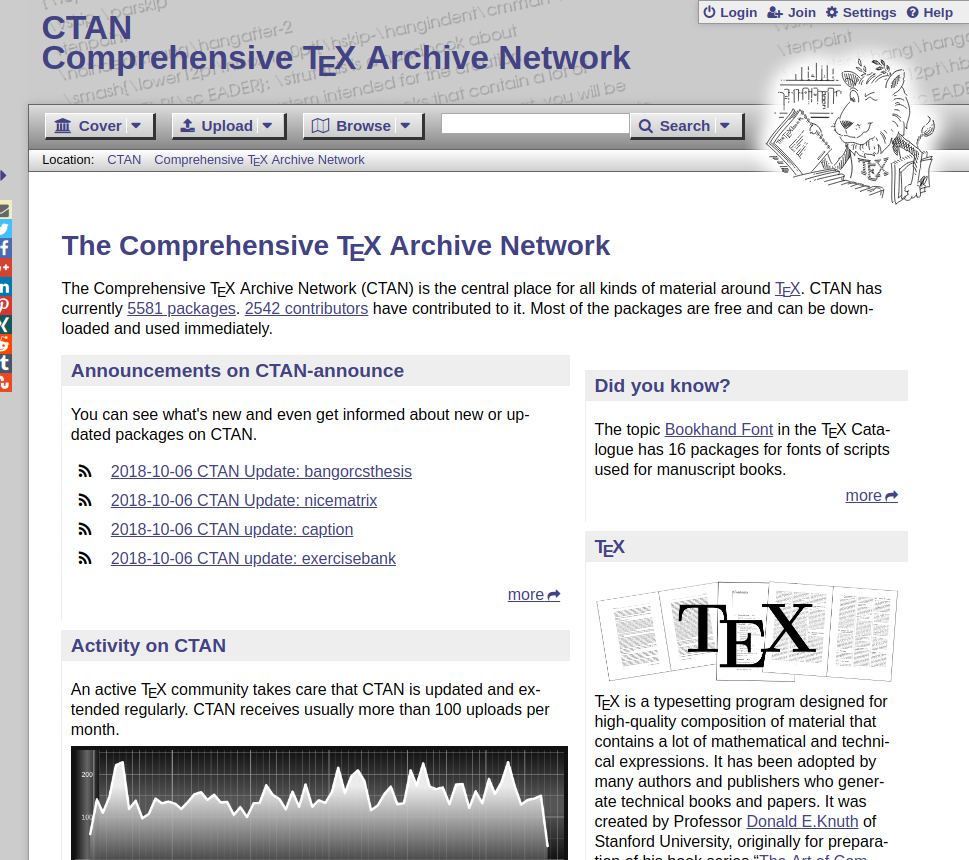
\includegraphics[width=\linewidth]{ctan.png}
			\end{columns}
				}
	
		\frame{\frametitle{When in doubt: Google}
			\begin{center}
			\only<1-3>{\TeX\ is older than the Happy Meal.\\}
			~\\
			\only<1>{~\\~\\}
			\only<2-3>{Someone has likely experienced your pain.\\}
			~\\
			\only<2>{~\\}
			\only<3>{\href{https://tex.stackexchange.com/}{https://tex.stackexchange.com/}}
			\end{center}
			}
	
		\frame{\frametitle{At your local library}
			\begin{block}{OU libraries has a \LaTeX\ expert:}
				\begin{columns}[onlytextwidth,T]
					\column{\linewidth-30mm-5mm}
						~\\~\\
						\textbf{Amanda Schilling}\\

						\faChain: \href{https://libraries.ou.edu/departments/stem-services}{Stem Services}
						
						\faPhone: (405) 325-6126
						
						\faEnvelope: \href{mailto:amanda.schilling@ou.edu}{amanda.schilling@ou.edu}
						
						~\\
						
						\textbf{Office Hours:} W/Th 8-9am in DAVIS\\
						\qquad\qquad M 6-8pm in the Learning Lab
						
					\column{30mm}
						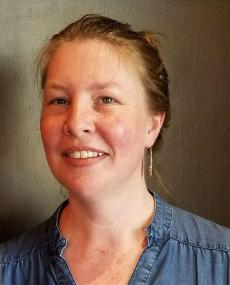
\includegraphics[width=30mm]{amanda.jpg}
				\end{columns}
			\end{block}
			}
		
		
			\frame{\frametitle{At your local library}
			\begin{block}{OU libraries has a \LaTeX\ expert:}
				\begin{columns}[onlytextwidth,T]
					\column{\linewidth-30mm-5mm}
					~\\~\\
					\textbf{Mark Laufersweiler}\\
					
					\faChain: \href{https://libraries.ou.edu/users/mark-laufersweiler}{Research Data Specialist}
					
					\faPhone: (405) 325-3710
					
					\faEnvelope: \href{mailto:laufers@ou.edu}{laufers@ou.edu}
					
					\column{30mm}
					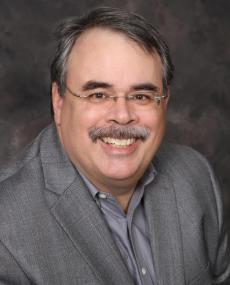
\includegraphics[width=30mm]{mark.jpg}
				\end{columns}
			\end{block}
		}
	
		\frame{\frametitle{Or contact me}
			\begin{block}{I'm just a \LaTeX\ junkie:}
				\begin{columns}[onlytextwidth,T]
					\column{\linewidth-30mm-5mm}
					~\\~\\
					\textbf{Wesley T. Honeycutt}\\
					
					\faChain: \href{wesleythoneycutt.com}{Personal Site}
					
					\faPhone: \emph{I have an office phone?}
					
					\faEnvelope: \href{mailto:honeycutt@ou.edu}{honeycutt@ou.edu}
					
					\faGithub: \href{https://github.com/BlueNalgene}{https://github.com/BlueNalgene}
					
					\column{30mm}
					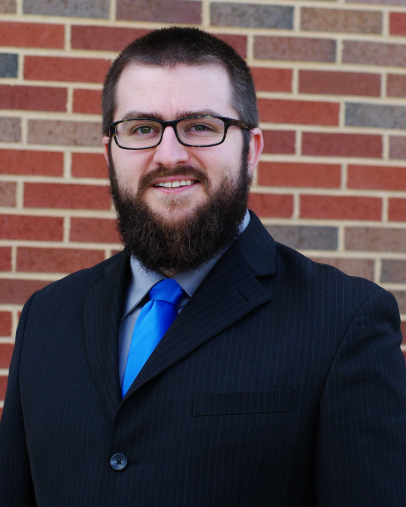
\includegraphics[width=30mm]{wes.png}
				\end{columns}
			\end{block}
			}
	
		\frame[containsverbatim]{ 
			\begin{LTXexample} 
				\begin{itemize} 
					\item First. 
					\item Second.
					\item Third.
				\end{itemize} 
			\end{LTXexample}
			
			\begin{LTXexample} 
				\begin{equation} 
					x^2 + y^2 = z^2. 
				\end{equation} 
			\end{LTXexample} 
			}
	
	
	
	

	
\end{document}